\chapter{User Manual}

\section{Introduction}

\textbf{Purpose: }

The purpose of this system is to give users a friendly experience when learning the trigonometry, pythagoras and vector aspects of maths, most likely as part of their GCSE preparation. The user can view lessons which provide sufficient knowledge to be able to gain some understanding of the topics, which they can then test using the homework provided. They can view their scores which are a reflection of their ability and progress in the subject. The end goal is that they do well in their maths GCSE, and this program is designed to help them do that.

\textbf{Intended Audience: }

The audience my program is targeting is GCSE students, in years 10 and 11 in the British education system (because this system is tailored more specifically to the syllabus of British exam boards) who have begun to prepare for their GCSE maths exam. Mainly year 10's are targeted as they will still be learning the basics of trigonoemtry, whereas year 11's should already know most of the subject, yet this system could still help them revise. Teachers could also be considered a client for this system as they might wish to use it in the school at which they are employed. Even parents of GCSE students or younger could be a client if they wished to provide their children with access to this system to boost their maths skills.

\section{Installation}

\subsection{Prerequisite Installation}

This system has been compiled to a windows executable (.exe) so no alternative software prerequisites are required to make use of this system on a windows operating system. Other operating systems have not been tested or developed for, so a windows operating system is required, preferably any of Windows 7, 8, or 10.

The following hardware list represents the minimum amount of hardware needed to be able to access and use every feature in the system:

\begin{itemize}
	\item A keyboard and a mouse for input 
	\item A visual display unit, preferably at least 20 inches wide, for all of the widgets to be properly visible and not over-lapping
	\item A hard disk drive (HDD) for storage
	\item A minimum of 512 megabytes of main memory (RAM) to perform processing
	\item An internet connection to download the software packages required to run the system (Python 3.4, PyQt4)
\end{itemize}

\subsubsection{Installing Python}

1. To install the appropriate version of Python (in order to be sure that it will be compatible), firstly go to \url{https://www.python.org/downloads/}.

\begin{figure}[H]
    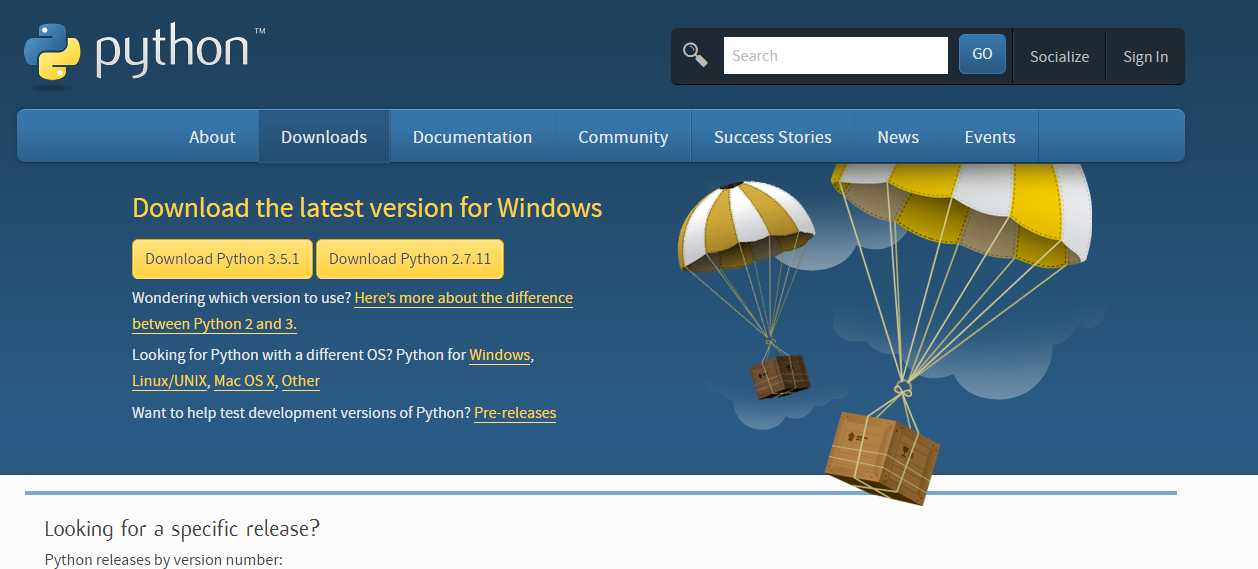
\includegraphics[width=\textwidth]{C:/Users/Jordan/git/COMP4Coursework2/Manual/install_python_1}
\end{figure}

2. Click on the first big yellow button titled \textbf{Download Python 3.5.1} (or whatever updated version) if you want the latest version of Python. \textbf{Be aware, you will have to find a compatible version of PyQt elsewhere, as not all versions are on the same website as the one intended for this version of Python.}

\begin{figure}[H]
    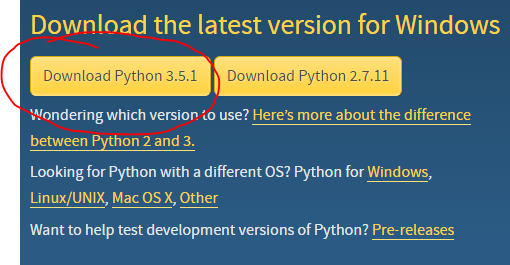
\includegraphics[width=\textwidth]{C:/Users/Jordan/git/COMP4Coursework2/Manual/install_python_2}
\end{figure}

3. Alternatively, scroll down to the list of past Python releases and click the one that says \textbf{Python 3.4.3 - 2015-02-25}, to use the version which the system was created with. 

\begin{figure}[H]
    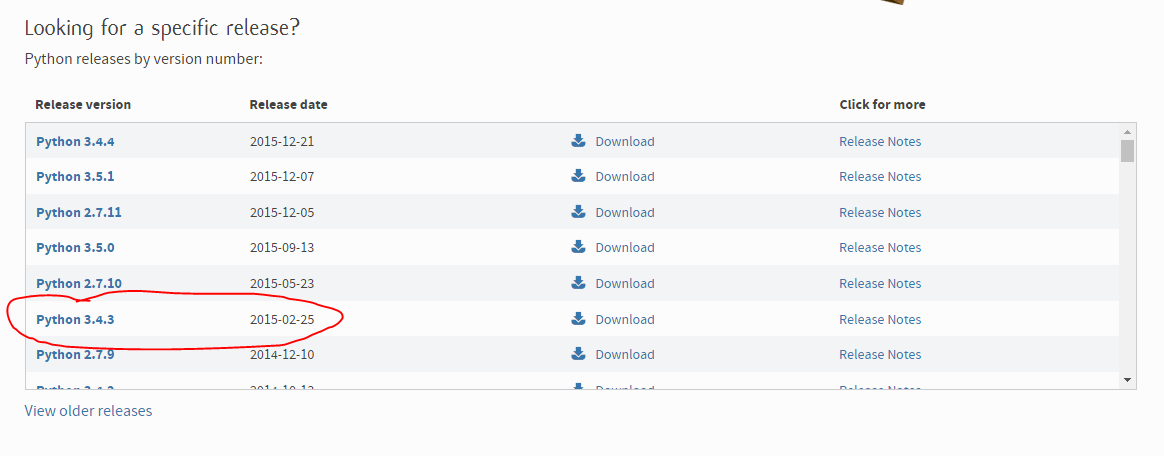
\includegraphics[width=\textwidth]{C:/Users/Jordan/git/COMP4Coursework2/Manual/install_python_3}
\end{figure}

4. If you chose the most recent version, the download will begin at the bottom of your window, and should take no longer than 1 minute depending on your internet connection speed.

\begin{figure}[H]
    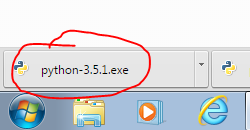
\includegraphics[width=\textwidth]{C:/Users/Jordan/git/COMP4Coursework2/Manual/install_python_4}
\end{figure}

5. Click the button with the download on it - A security warning will pop up. This file, presuming you selected the right one using the instructions above, is safe, so click run. Then a new window will open. \textbf{Please skip to step 8.}

\begin{figure}[H]
    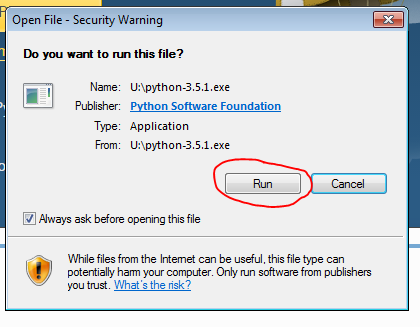
\includegraphics[width=\textwidth]{C:/Users/Jordan/git/COMP4Coursework2/Manual/install_python_5}
\end{figure}

\begin{figure}[H]
    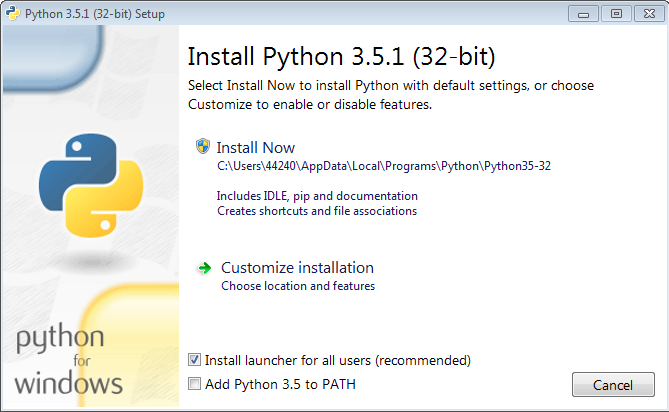
\includegraphics[width=\textwidth]{C:/Users/Jordan/git/COMP4Coursework2/Manual/install_python_6}
\end{figure}

6. If you selected a past version, a different window will open in your internet browser. Click on the \textbf{Windows x86 MSI Installer} for Windows. The download will begin at the bottom of your window, and should take no longer than 1 minute depending on your internet connection speed. Click on the button, and a similar window to the other version will open.

\begin{figure}[H]
    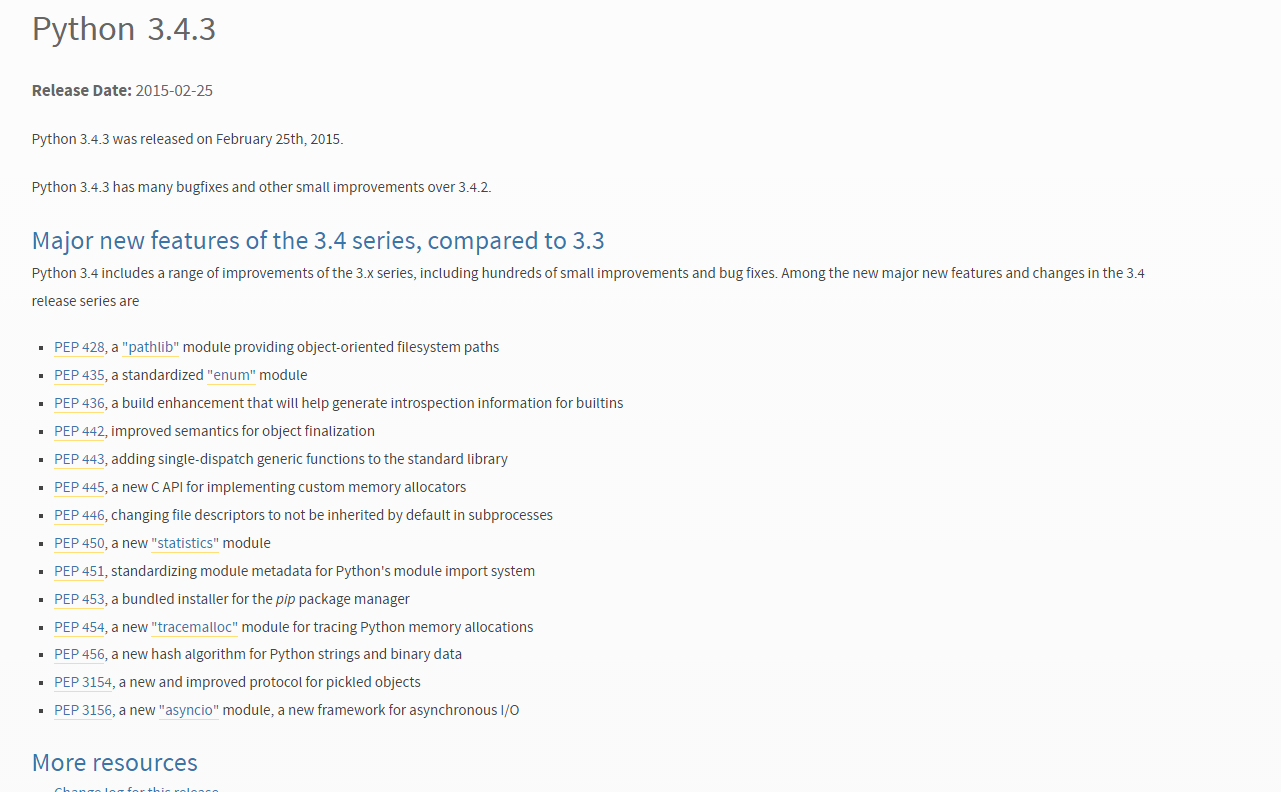
\includegraphics[width=\textwidth]{C:/Users/Jordan/git/COMP4Coursework2/Manual/install_python_7}
\end{figure}

\begin{figure}[H]
    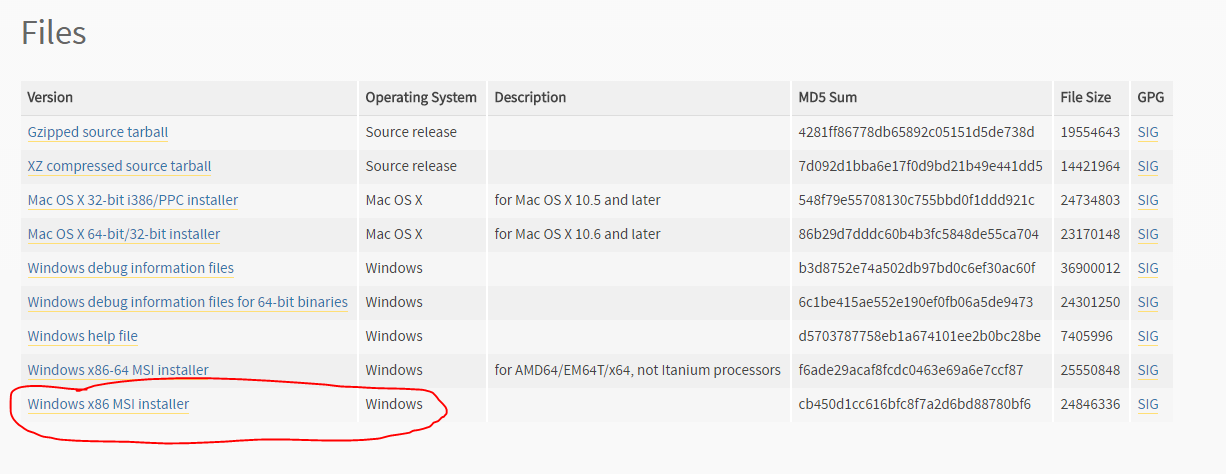
\includegraphics[width=\textwidth]{C:/Users/Jordan/git/COMP4Coursework2/Manual/install_python_8}
\end{figure}

\begin{figure}[H]
    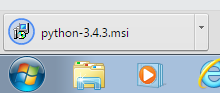
\includegraphics[width=\textwidth]{C:/Users/Jordan/git/COMP4Coursework2/Manual/install_python_9}
\end{figure}

7. A security warning will pop up. This file, presuming you selected the right one using the instructions above, is safe, so click run.

\begin{figure}[H]
    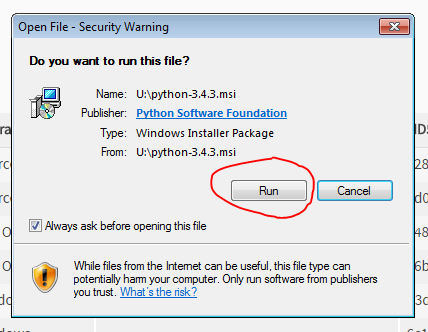
\includegraphics[width=\textwidth]{C:/Users/Jordan/git/COMP4Coursework2/Manual/install_python_10}
\end{figure}

8. A setup wizard window will open (for whichever version of Python you chose). It is recommended that you leave install for all users ticked and click next.

\begin{figure}[H]
    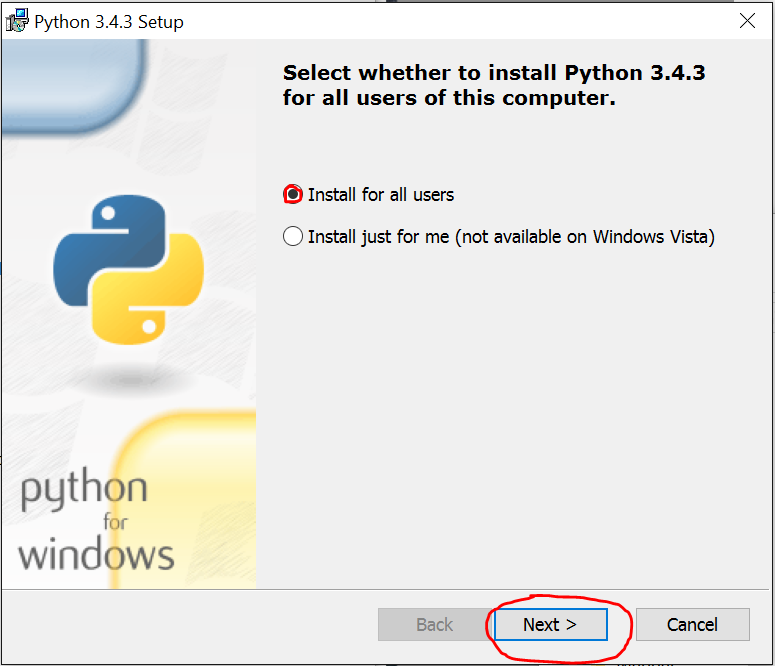
\includegraphics[width=\textwidth]{C:/Users/Jordan/git/COMP4Coursework2/Manual/install_python_11}
\end{figure}

9. A directory should already be selected, most likely in your C: drive. This is an ideal place to save the Python files, but if you would prefer that they were saved somewhere else then click the 'Up' button to search through alternative locations. Once your directory has been selected, click next to continue.

\begin{figure}[H]
    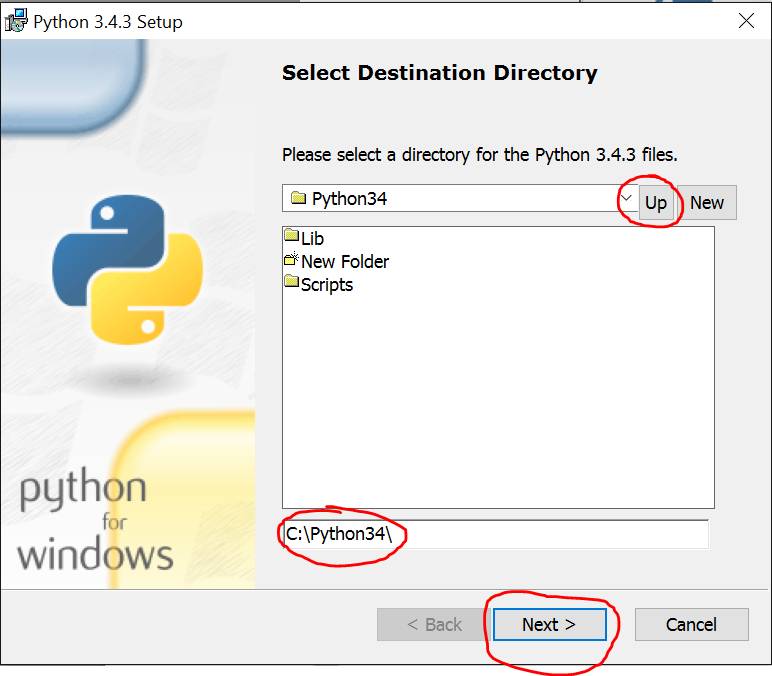
\includegraphics[width=\textwidth]{C:/Users/Jordan/git/COMP4Coursework2/Manual/install_python_12}
\end{figure}

10. On the next window, most of the settings should be left alone. It might be useful however to add python to your path by selecting the bottom option, \textbf{Add python.exe to Path}, and choosing the first option, \textbf{Will be installed on local hard drive}. However this is not essential for using the system. Once you have decided on these settings click next.

\begin{figure}[H]
    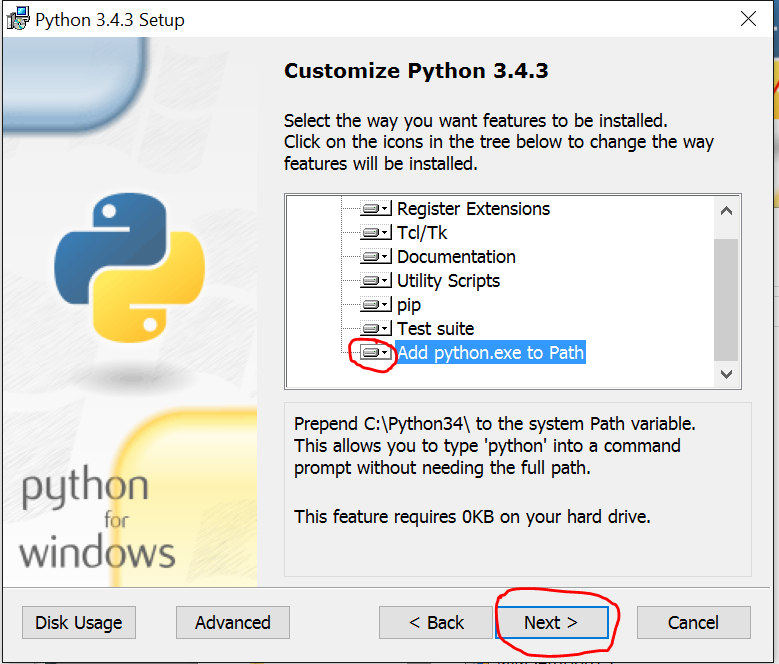
\includegraphics[width=\textwidth]{C:/Users/Jordan/git/COMP4Coursework2/Manual/install_python_13}
\end{figure}

11. When you are asked if you would like to allow the system to make changes to your computer, click yes. Then wait a minute for Python to install. Once it has finished, click finish. Now Python is on your computer and ready to use.

\begin{figure}[H]
    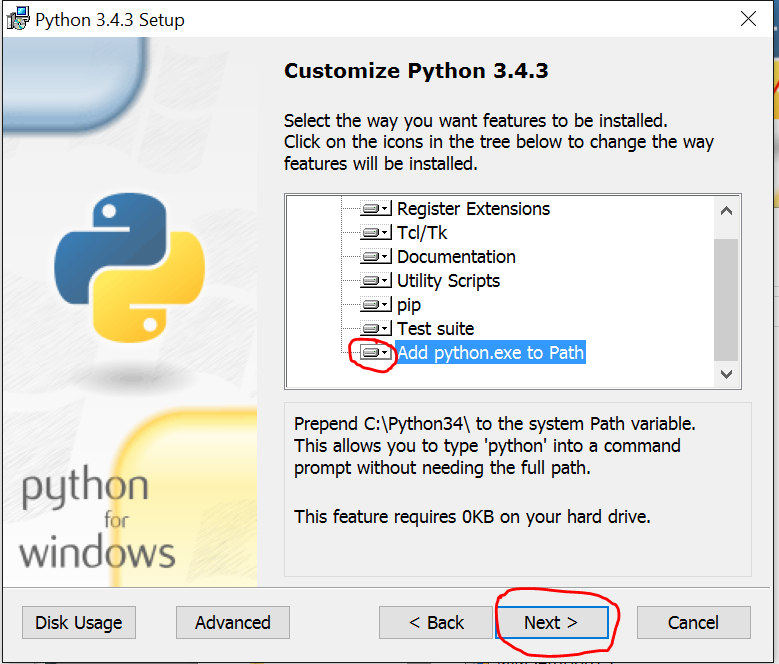
\includegraphics[width=\textwidth]{C:/Users/Jordan/git/COMP4Coursework2/Manual/install_python_13}
\end{figure}

\subsubsection{Installing PyQt4}

1. To install PyQt4 (not PyQt5 as it won't be compatible with the system), firstly go to \url{https://riverbankcomputing.com/software/pyqt/download}.

\begin{figure}[H]
    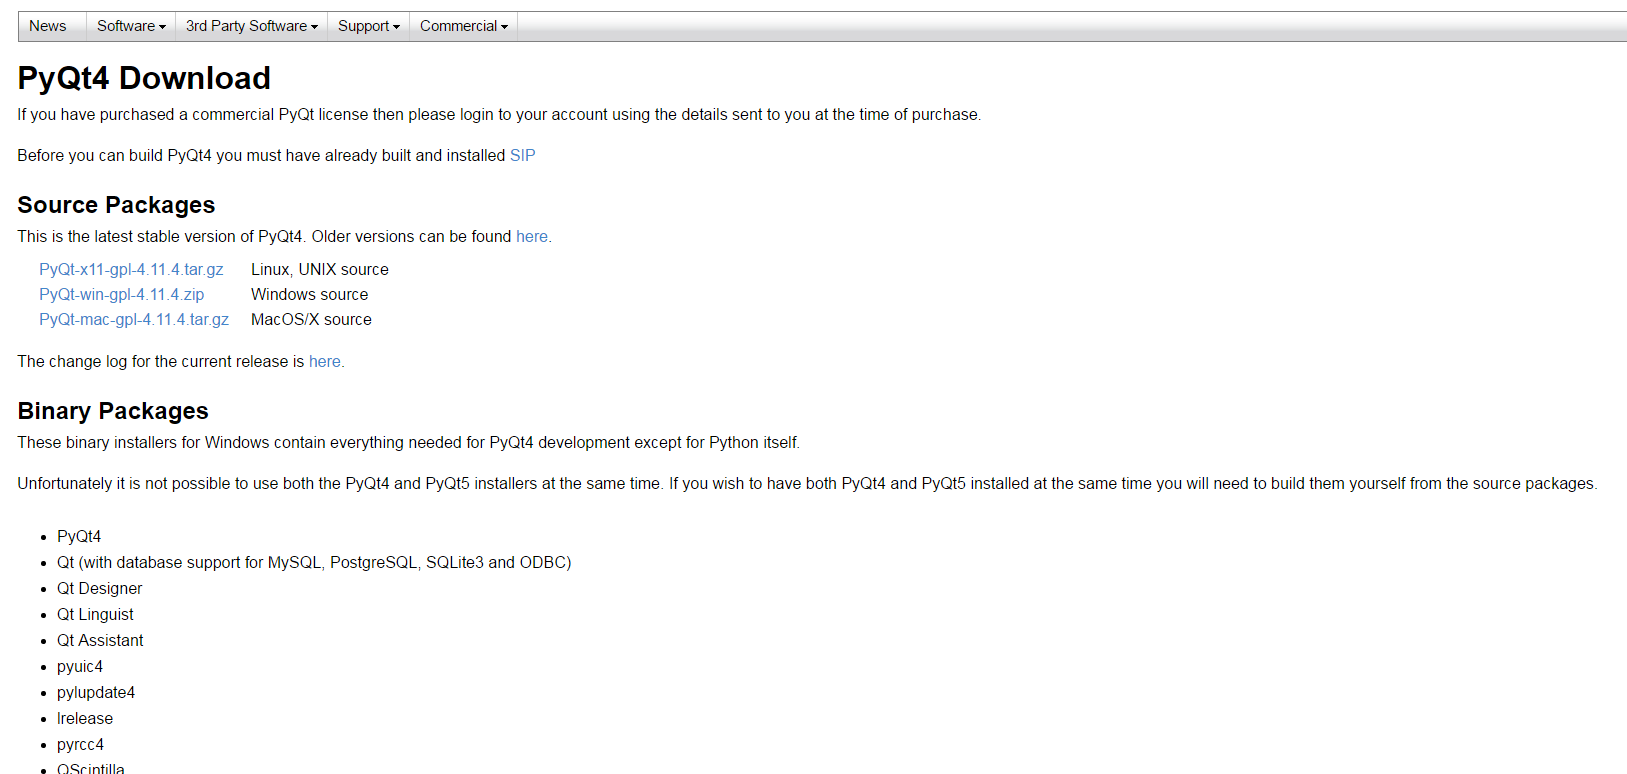
\includegraphics[width=\textwidth]{C:/Users/Jordan/git/COMP4Coursework2/Manual/install_pyqt_1}
\end{figure}

2. This system is designed to run on a 32 bit version of Python, so choose the \textbf{PyQt4-4.11.4-gpl-Py3.4-Qt4.8.7-x32.exe} file for the Windows 32-bit installer.

\begin{figure}[H]
    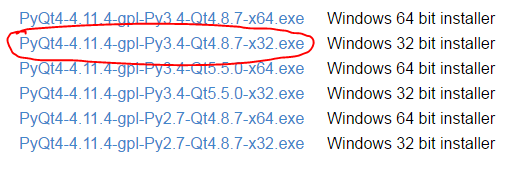
\includegraphics[width=\textwidth]{C:/Users/Jordan/git/COMP4Coursework2/Manual/install_pyqt_2}
\end{figure}

3. When you click on the link a new window will open in your browser telling you your download will begin shortly. Give it a few seconds and you should see the download button appear in the bottom left corner of the window.

\begin{figure}[H]
    
\includegraphics[width=\textwidth]{C:/Users/Jordan/git/COMP4Coursework2/Manual/install_pyqt_3}
\end{figure}

\begin{figure}[H]
    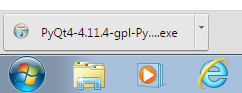
\includegraphics[width=\textwidth]{C:/Users/Jordan/git/COMP4Coursework2/Manual/install_pyqt_4}
\end{figure}

4. Click the button and an install wizard window will open. Click the next button to begin setting up PyQt4.

\begin{figure}[H]
    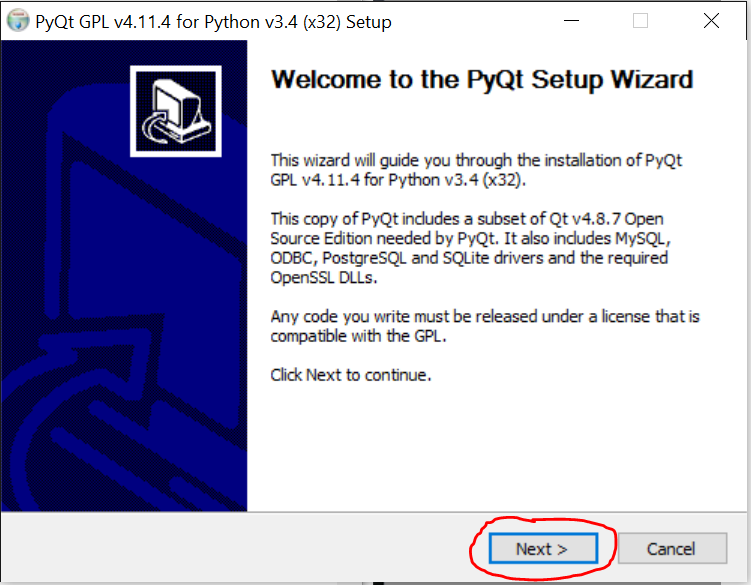
\includegraphics[width=\textwidth]{C:/Users/Jordan/git/COMP4Coursework2/Manual/install_pyqt_5}
\end{figure}

5. Click the 'I Agree' button to accept the terms and conditions of the PyQt4 software package - assuming you've found the right package using the instructions, it is perfectly safe.

\begin{figure}[H]
    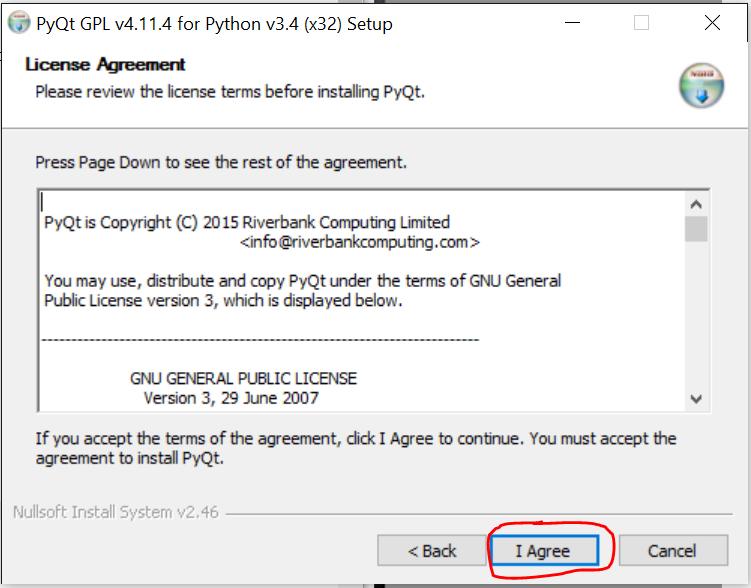
\includegraphics[width=\textwidth]{C:/Users/Jordan/git/COMP4Coursework2/Manual/install_pyqt_6}
\end{figure}

6. Everything that comes with the software package is ticked for you by default - do not untick anything, as it may be something required to run the system. Leave the check boxes as they are and click next.

\begin{figure}[H]
    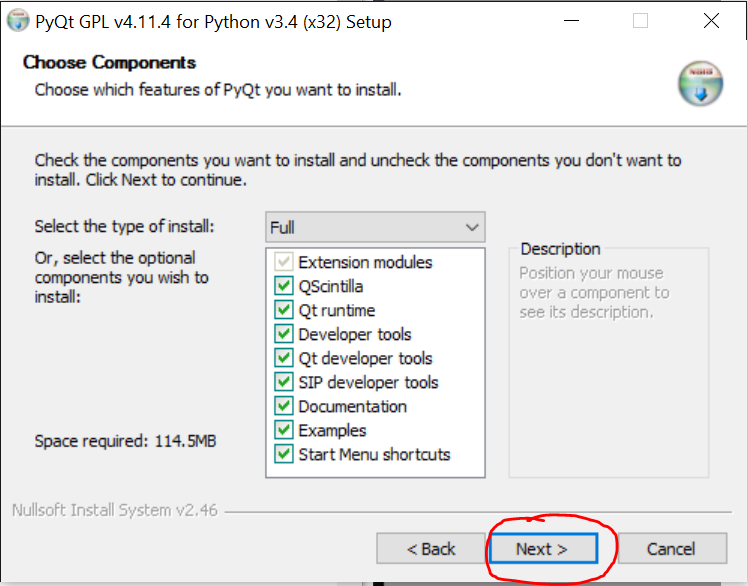
\includegraphics[width=\textwidth]{C:/Users/Jordan/git/COMP4Coursework2/Manual/install_pyqt_7}
\end{figure}

7. The install wizard will ask you to select a folder for the PyQt4 files. It should have already selected your Python folder if you have installed Python already, in which case leave it and click install to ensure that the files are accessible by Python. If it does not already have a Python folder selected, it is recommended that you install Python first, or, if you have, search for Python in your file explorer and select Python 3 manually by clicking the browse button. Once you have Python3 selected, click install.

\begin{figure}[H]
    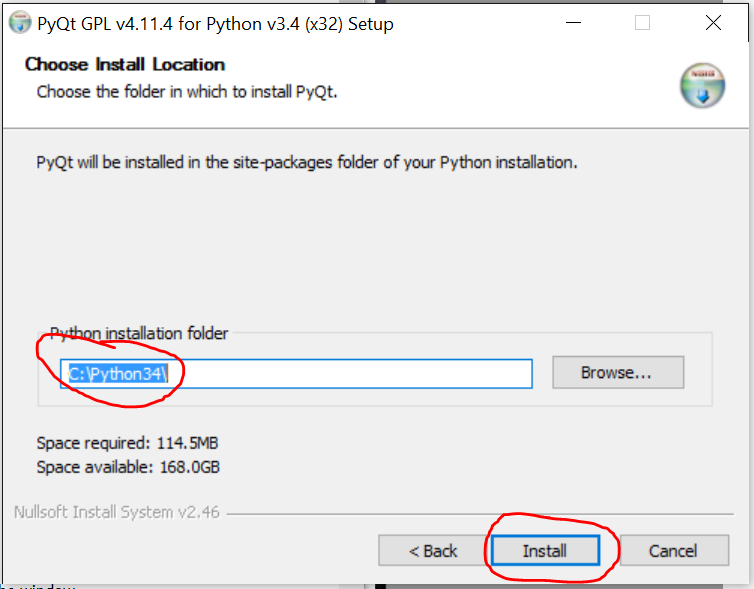
\includegraphics[width=\textwidth]{C:/Users/Jordan/git/COMP4Coursework2/Manual/install_pyqt_8}
\end{figure}

8. Wait one minute for the installation to finish, then click the finish button. PyQt4 will now be installed on your computer and ready to be used for the system.

\begin{figure}[H]
    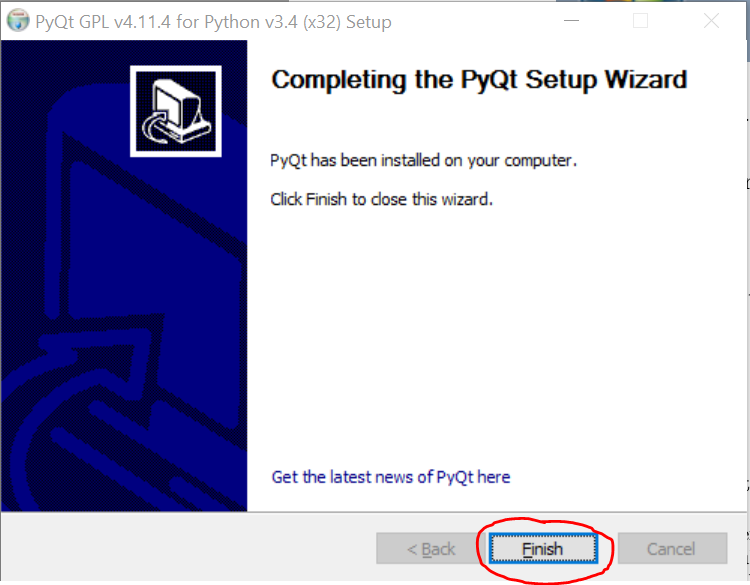
\includegraphics[width=\textwidth]{C:/Users/Jordan/git/COMP4Coursework2/Manual/install_pyqt_9}
\end{figure}

\subsection{System Installation}

1. Navigate to the directory where you placed the installer file.

\begin{figure}[H]
    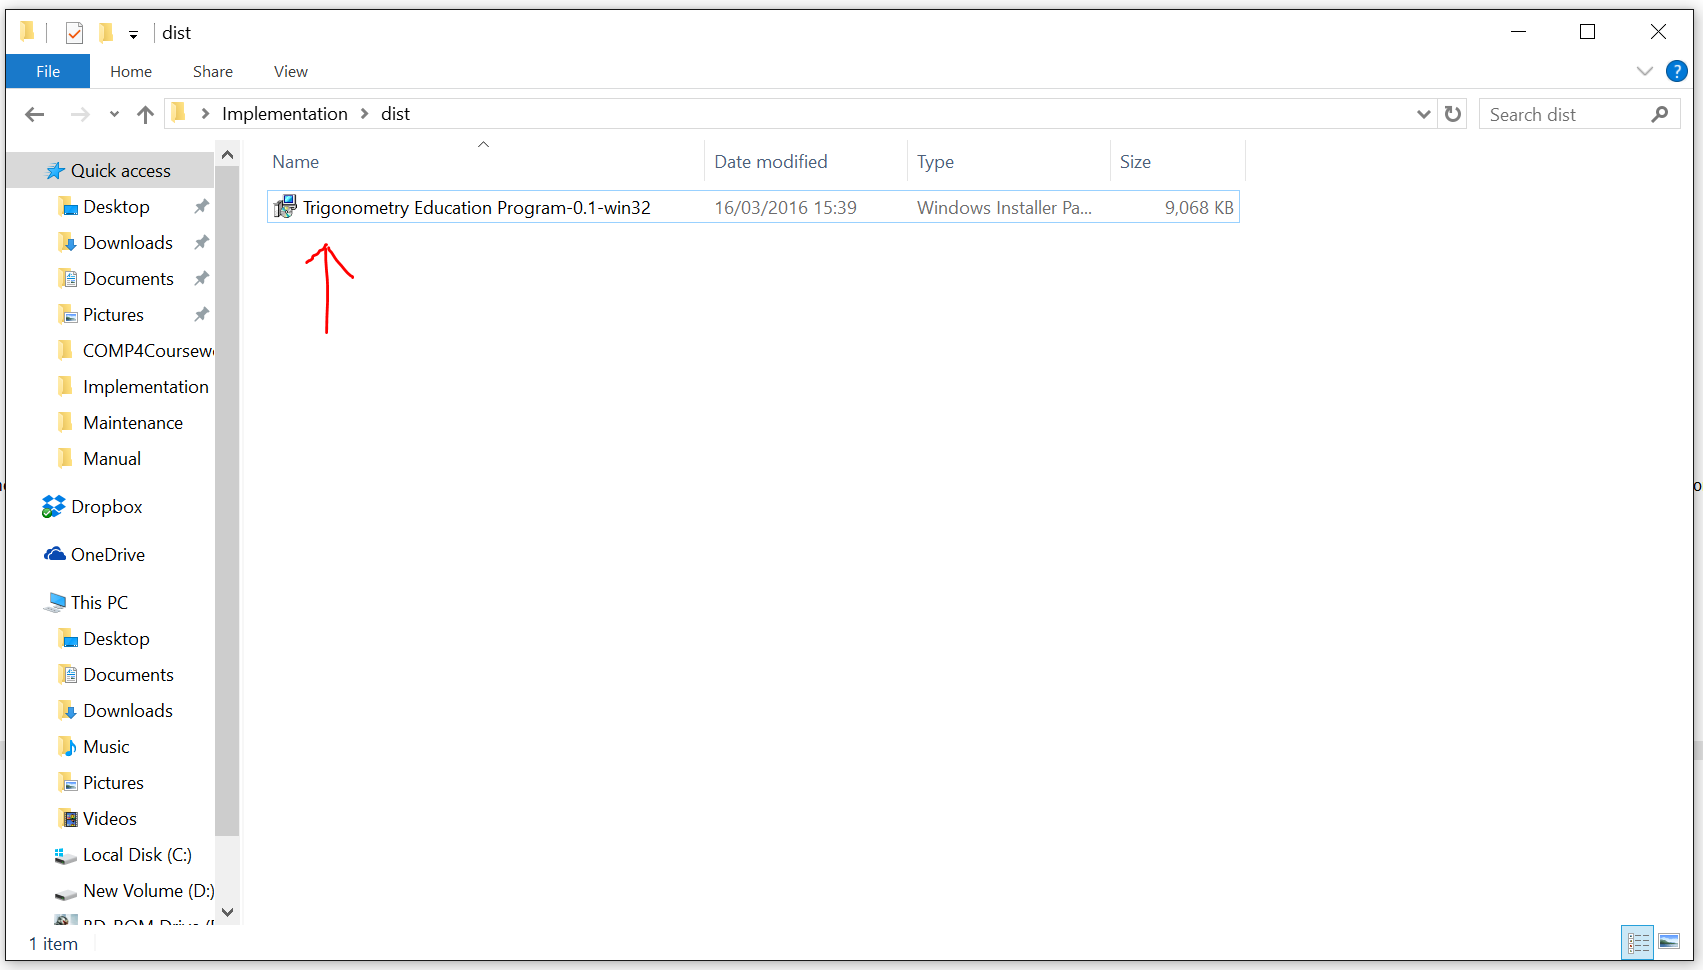
\includegraphics[width=\textwidth]{C:/Users/Jordan/git/COMP4Coursework2/Manual/install_system_1}
\end{figure}

2. Double click with the left mouse button on the installer to start the installation process. You will be asked to choose a location to install the system. It is recommended that you go with the default recommendation, but otherwise you can use the arrows to navigate to a different directory. Once you have selected a directory, click next.

\begin{figure}[H]
    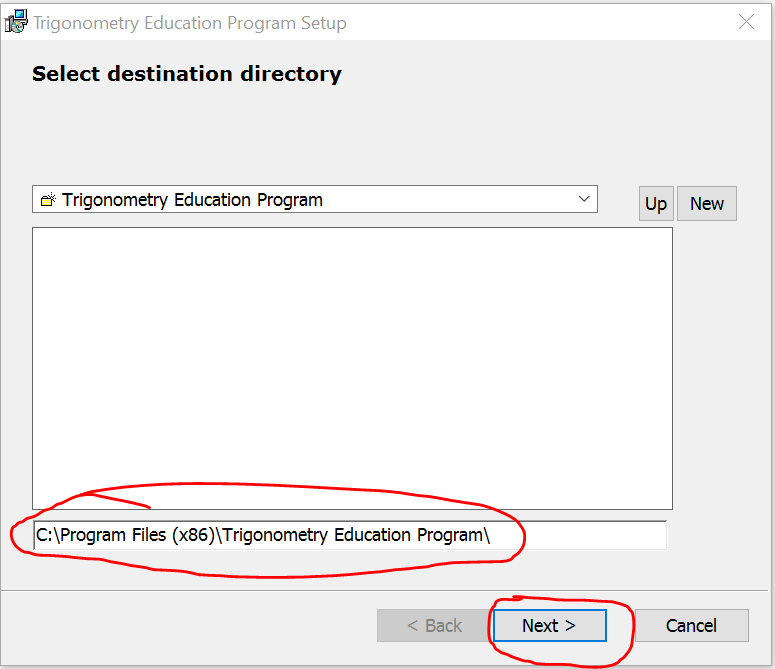
\includegraphics[width=\textwidth]{C:/Users/Jordan/git/COMP4Coursework2/Manual/install_system_2}
\end{figure}

3. A security window will ask whether you want to allow the system to make changes to your computer. Click yes, then wait a few seconds for the system to install. Finally click finish, and the program will be installed on your computer ready for use.

\begin{figure}[H]
    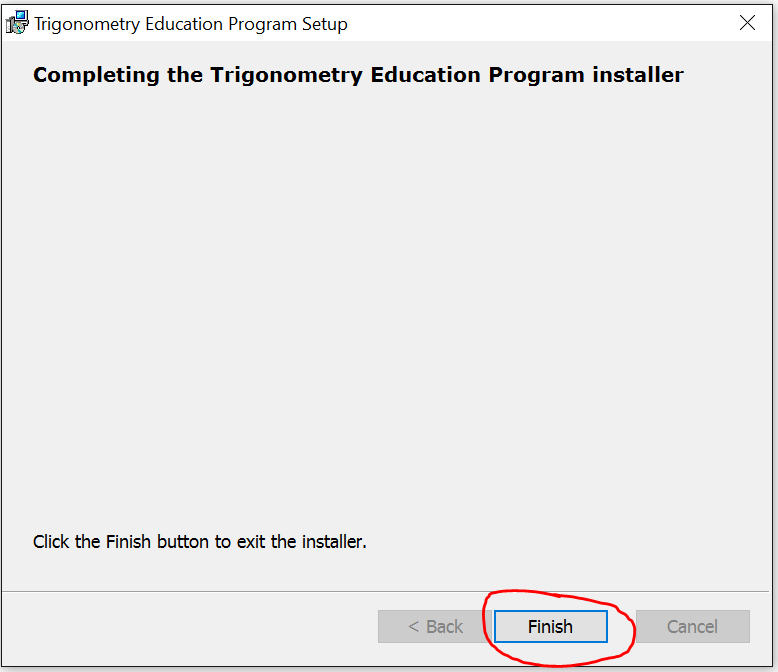
\includegraphics[width=\textwidth]{C:/Users/Jordan/git/COMP4Coursework2/Manual/install_system_3}
\end{figure}

\subsection{Running the System}

\textbf{Make sure you have installed the system first by using the instructions in section 5.2.2}

1. Navigate to the directory where you installed the system files previously. It will run the same way wherever it has been saved, as long as the file \textbf{student\_database.db} is in the same folder as the application file.

\begin{figure}[H]
    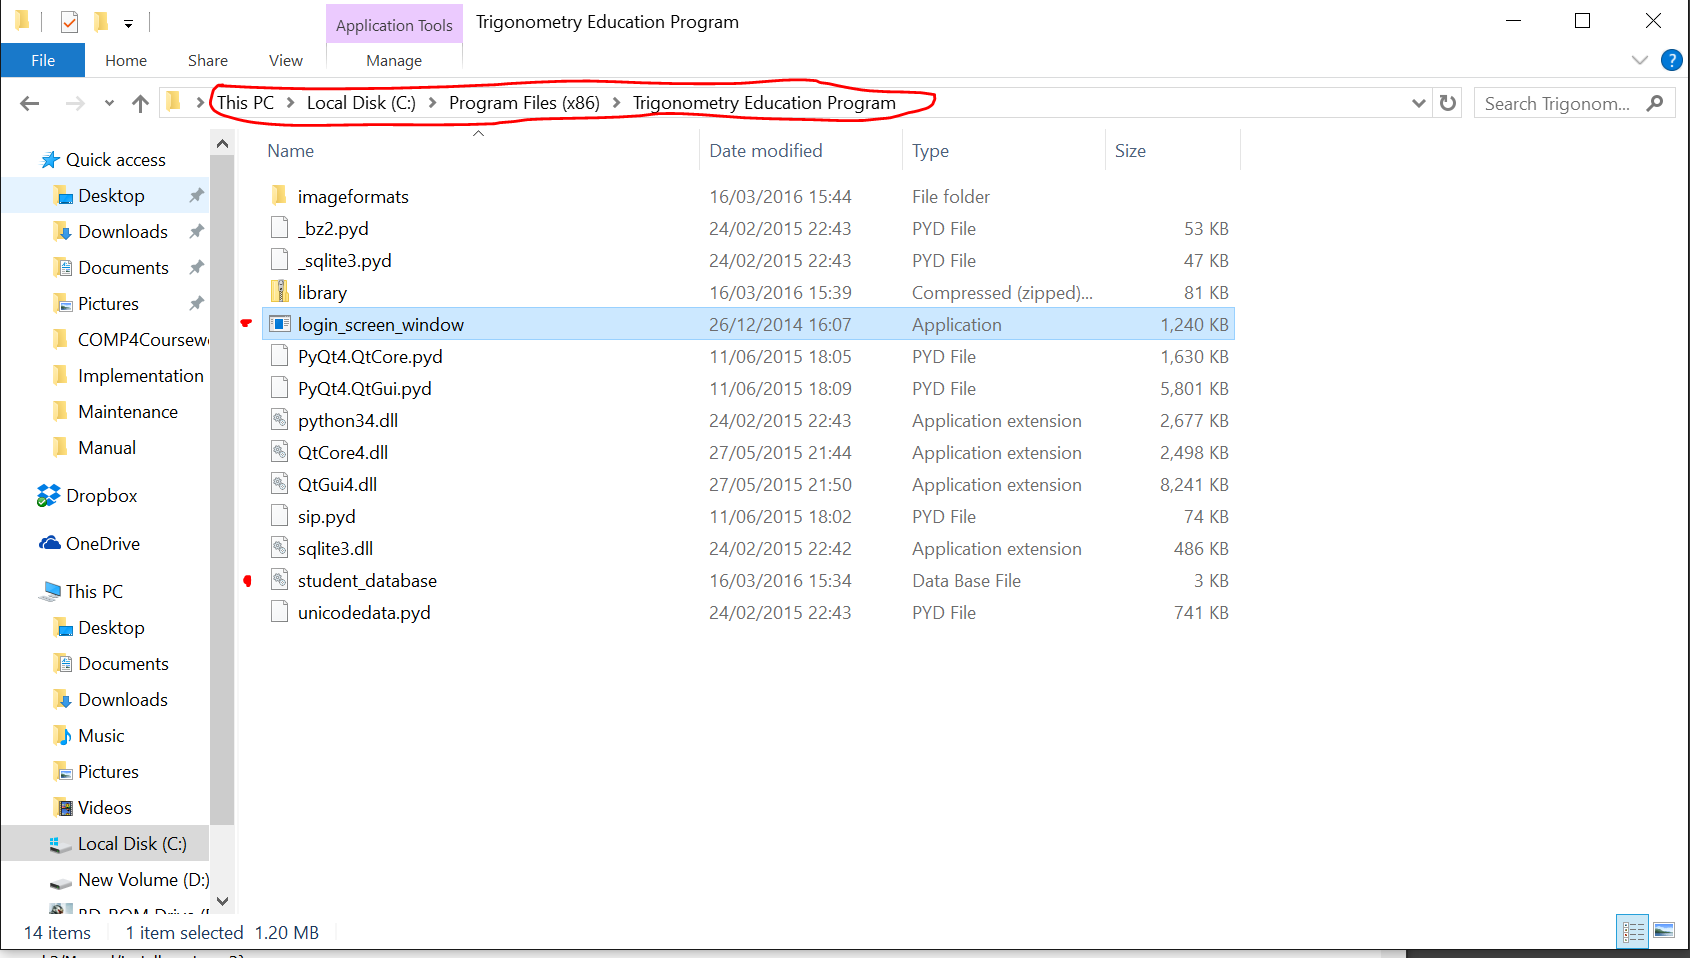
\includegraphics[width=\textwidth]{C:/Users/Jordan/git/COMP4Coursework2/Manual/run_system_1}
\end{figure}

2. Double click on the application file title \textbf{Trigonometry Education Program} to start running the system.

3. The system will load and appear on the screen. It is now running and can be used as desired.

\begin{figure}[H]
    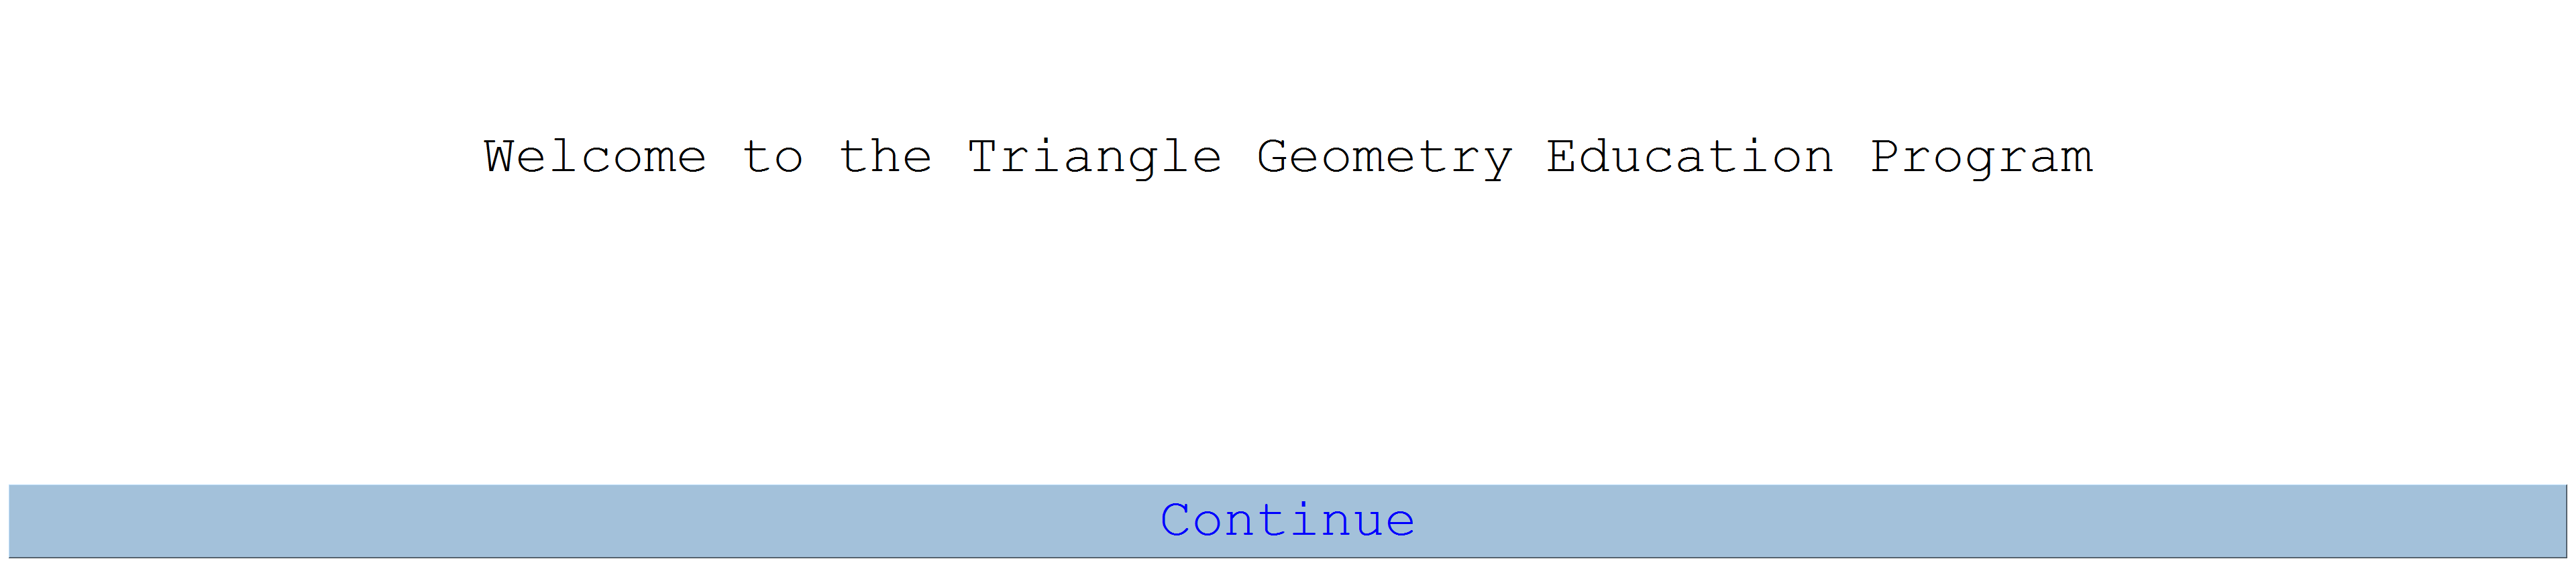
\includegraphics[width=\textwidth]{C:/Users/Jordan/git/COMP4Coursework2/Manual/run_system_2}
\end{figure}

\section{Tutorial}

\subsection{Introduction}

In this section I will explain how to use each aspect of the system in order for the user to gain the full benefits of its purpose; using this guide the user should have no problems with the system which they will not be able to easily deal with. Each aspect will be explained using detailed instructions and annotated images to assist the user in understanding each aspect of the system.

\subsection{Assumptions}

The assumption that the user has basic computer capabilities and can use the mouse and keyboard has been made, and that the system is already running and ready for the user to use. Otherwise, things like the navigation of the system and the functions available to use in the system have not been assumed as known by the user.





\subsection{Tutorial Questions}

\subsubsection{How do I access the lessons?}

To access the lessons there is a branch system of menus which can be followed down to a lesson. From the home screen (pictured below) click the lessons button, then use the names on the buttons in the next menu to find the lesson which you want to use. The names of the sub menus are relevant to the lesson topics accessible from that sub menu. For example, to find the Pythagoras lessons, click the Pythagoras button and the Pythagoras Theorem lesson will be accessible from that sub-menu.

%Screenshots

Upon clicking a lesson button the lesson window will open.

%Screenshot of lesson screen

\subsubsection{How do I access the homework?}

Accessing the homework uses essentially the same system as accessing the lessons, only there are more options to choose from on the sub-menus. For each lesson, there are three homework tasks of varying difficulty. Starting from the home screen, click on the homework button (pictured below).

%Screenshot of home screen

From the homeork topic menu, choose a topic related to the homework you wish to complete, and the sub-menu with the button to open that homework will open. If it is the wrong sub-menu, simply press return and try the other menus. Clicking the button with the title of the homework you want to complete will open that homework.

%Screenshot sub-menu then homework screen

\subsubsection{How do I view my progress?}

To view all of the information stored in the database, from the home screen (pictured below) click the progress button.

%Screenshot of home with progress button circled

All of the information will immediately be displayed in the progress window which will open upon clicking the progress button.

%Screenshot of progress window

\subsubsection{How can I look at specific details of my progress?}

From the progress screen, accessed by clicking the progress button on the home screen, click on the report button to open a new window.

%Screenshot of progress screen with report button circled

The first combo box contains all the names of the tasks. Click on the arrow, and select the name of the task which you want to query the database for. Then do the same with the next combo box, only this time you are choosing the score you want to query. You can choose to query one or the other by leaving the input blank. Once you have chosen your query criteria, click on the submit button and the relevant information will appear in the table to the left.

%Screenshot of combo box with stuff in table

\subsubsection{How do I know I won't lose progress by exiting the program?}

The only way you could lose progress is by closing a homework window using the cross in the top right hand corner of the window instead of using the next or finish button - only the inputs on those screen will be lost, and you will have to put them in again if you want the saved results. As long as the next or finish button is clicked, the progress from the respective page will be saved automatically by the system. Progress already stored in the database can only be lost if it is over-written with better results, or if you manually delete the \textbf{student\_database.db} file. Otherwise, information in the database will not delete itself at any point.

%Screenshot with cross as x - no, and next and finish buttons

\subsubsection{How do I save my progress?}

You do not need to manually save anything. The only way to save results is by clicking the next button on a homework first page, to save the first half of a record, then by clicking the finish button on a homework second page, to save the second half of a record. All saves will be made internally and automatically, and all new information will immediately be available for viewing in the progress window or the report window.

%Screenshots of next and finish buttons and new info in progress window

\subsubsection{What do I do if an error message pops up?}

Details on how to deal with specific error messages are in section 5.4, but in order to remove an error message window from the centre of the screen you must simply click the OK button and then proceed to do what the error message advised you do.

%Screenshot of error message appearing after wrong thing then closing it.






\subsection{Saving}

There is only one file saved and accessed by the system and that is the \textbf{student\_database.db} file. All saving is done internally and automatically by the system; when the user clicks next on a homework first page window, the task name and first question score is saved, then when they click finish on the second homework screen, the other question scores are updated on the record just saved prior to opening this screen. The methods run when the buttons are clicked will automatically execute a database query, so the user does not have to manually save anything, just complete all of the questions and close the stack window using the finish button, not the cross in the top right corner of the window.

\subsection{Limitations}

The database cannot be reset by the user in-system. This was a secondary objective considered which did not make it into the system, so unless it is updated in the future the only way a user would be able to reset all of their progress would be to manually delete the \textbf{student\_database.db} file from their system files. Upon running the program a new database would be created with the same name, and it would be initially empty.

The system does not have any of the administrative capabilities originally proposed in the analysis, essentially meaning that the client on this case will not be able to monitor students' progress, although they will still have the same level of opportunity to gain knowledge of the relevant aspects of maths in preparation for their GCSE's.





\section{Error Recovery}

\subsection{ErrorMessage2}

This error message appears if the user inputs a wrong data type for an answer - it is essentially a friendly way of giving them another go because they made quite a big mistake, not just a wrong answer of the right data type, without removing an attempt.

%Screenshot of error message

To solve this error, simply go back to the same input box which the wrong answer was typed into, and try again using a decimal value - a number with a point before and after at least 1 digit. For example, 4.5 or 7.13.

\subsection{ErrorMessage3}

This error message appears if the user inputs a wrong data type for an answer - it is essentially a friendly way of giving them another go because they made quite a big mistake, not just a wrong answer of the right data type, without removing an attempt.

%Screenshot of error message

To solve this error, simply go back to the same input box which the wrong answer was typed into, and try again using an integer - a whole number such as 5 or 120.

\subsection{ErrorMessage4}

This error message appears if the user inputs a wrong data type for an answer - it is essentially a friendly way of giving them another go because they made quite a big mistake, not just a wrong answer of the right data type, without removing an attempt.

%Screenshot of error message

To solve this error, simply go back to the same input box which the wrong answer was typed into, and try again using a string - a word or answer consisting of letters like 'triangle'.

\subsection{ErrorMessage5}

This error message just informs the user that they got an answer incorrect so they know to have another go, if they have attempts remaining. To deal with this error simply try again until either you get it right or run out of attempts.

%Screenshot of error message

\subsection{ErrorMessage8}

This error message appears if the user has not answered and checked all of the questions on a homework. If this message appears, find the input box which you have not yet attempted, check your input until you get it right or run out of attempts, then you will be able to proceed to the next screen. The reason for this error is that a score value is required for the system to be able to execute the SQL query which saves the score to the database.

%Screenshot of error message






\section{System Recovery}

\subsection{Backing-up Data}

It is quite simple to back up the data for this system. There is only one file with data, and that will be called \textbf{student\_database.db} and is located in the {} folder in {}.

%Screenshot of file name

Left click on the \textbf{student\_database.db} file ONCE and then right click on it when it is highlighted.

%Screenshot of highlighted file name with menu box

In the menu box, select 'Copy'. Alternatively, when it is highlighted, hold Ctrl and press C.

%Screenshot of mouse hovering over copy

Now navigate to a folder separate from the folder the file is currently in, to avoid the backup also being lost should there be a fault with the folder. For example, {}.

%Screenshot of different folder

Now right click on a white space in the folder, and when the menu box appears, select 'Paste'.  Alternatively, hold Ctrl and press P.

%Screenshot of it pasted into new folder

Now you have a copy of the file with all of the database details on it, which can be accessed to replace the other copy should anything happen to it, like corruption or deletion. If you want to be even more secure you can upload a copy to Dropbox or a similar website.

\subsection{Restoring Data}

To restore the \textbf{student\_database.db} file, firstly navigate to where you pasted the copy of it from the backing-up data section. If you have not already done this, chances are you will not be able to get the file back at all.

%Screenshot of file.

Left click on the file to highlight it, then right click on it to make the menu box appear. Select the 'Copy' option. Alternatively, when it is highlighted, hold Ctrl and press C.

%Screenshot of copying

Now navigate to the folder where all of the system files are kept, where either the file you want to replace is or the deleted file was.

%Screenshot of folder

If a corrupt or unwanted file is there, left click on it to highlight it, then right click anywhere and select 'Paste'.  Alternatively, just hold Ctrl and press P when in the folder.

%Screenshot pasting

A window will appear asking you if you want to replace or duplicate the file. Click replace.

%Screenshot of window

If a file is not already there, just hold Ctrl and press P, and the copy will immediately be placed in the folder.

%Screenshot of pasted file

Your restored \textbf{student\_database.db} file is now in the folder ready to be used.

%Do at home for screenshots:

%Errors
%Questions
%System recovery - Screenshots
%{} Backing up data find file name - At home - compile program